\documentclass[aspectratio=169]{beamer}
% \usepackage{pgfpages}
% \pgfpagesuselayout{4 on 1}[a4paper,landscape,border shrink=5mm]
\usepackage{tikz}
\usetikzlibrary{shapes, backgrounds, arrows, positioning}
%\usepackage{pgfplots}
\usepackage{listings}
\usepackage[utf8,latin1]{inputenc}
\usepackage[style = apa, backend = biber, natbib = true]{biblatex}
\addbibresource{../../literature/lit.bib}

\makeatletter \def\newblock{\beamer@newblock} \makeatother  

\beamertemplatenavigationsymbolsempty
\setbeamertemplate{itemize items}[circle]
\setbeamertemplate{section in toc}[circle]
\mode<beamer>{\setbeamercolor{math text displayed}{fg=iwmgray}}
\setbeamercolor{block body}{bg=iwmorange!50!white}
\setbeamercolor{block title}{fg=white, bg=iwmorange}

% Definitions for biblatex
\setbeamercolor{bibliography entry note}{fg=iwmgray}
\setbeamercolor{bibliography entry author}{fg=iwmgray}
\setbeamertemplate{bibliography item}{}

\definecolor{iwmorange}{RGB}{255,105,0}
\definecolor{iwmgray}{RGB}{67,79,79}
\definecolor{iwmblue}{RGB}{60,180,220}
\definecolor{iwmgreen}{RGB}{145,200,110}
\definecolor{iwmpurple}{RGB}{120,0,75}

\setbeamercolor{title}{fg=iwmorange}
\setbeamercolor{frametitle}{fg=iwmorange}
\setbeamercolor{structure}{fg=iwmorange}
\setbeamercolor{normal text}{fg=iwmgray}
\setbeamercolor{author}{fg=iwmgray}
\setbeamercolor{date}{fg=iwmgray}

\title{Longitudinal data}
\author{Nora Wickelmaier}

\date{Last modified: \today}

\newcommand{\vect}[1]{\mathbf{#1}}
\newcommand{\mat}[1]{\mathbf{#1}}
\newcommand{\gvect}[1]{\boldsymbol{#1}}
\newcommand{\gmat}[1]{\boldsymbol{#1}}

\lstset{language = R,%
  basicstyle = \ttfamily\color{iwmgray},
  frame = single,
  rulecolor = \color{iwmgray},
  commentstyle = \slshape\color{iwmgreen},
  keywordstyle = \bfseries\color{iwmgray},
  identifierstyle = \color{iwmpurple},
  stringstyle = \color{iwmblue},
  numbers = none,%left,numberstyle = \tiny,
  basewidth = {.5em, .4em},
  showstringspaces = false,
  emphstyle = \color{red!50!white}}

\AtBeginSection[]{
  \frame{
    \tableofcontents[sectionstyle=show/hide, subsectionstyle=show/show/hide]}}

\setbeamertemplate{headline}{
 \begin{beamercolorbox}{section in head}
   \vskip5pt\insertsectionnavigationhorizontal{\paperwidth}{}{}\vskip2pt
 \end{beamercolorbox}
}

\setbeamertemplate{footline}{\vskip-2pt\hfill\insertframenumber$\;$\vskip2pt}

\begin{document}

\begin{frame}{}
\thispagestyle{empty}
\titlepage
\end{frame}

\begin{frame}{Outline}
\tableofcontents
\end{frame}

\section[Introduction]{Introduction mixed-effects models}

\begin{frame}{Mixed-effects models}
\begin{itemize}
  \item Mixed-effects models take account of dependencies in hierarchical,
    longitudinal, and other dependent data
  \item Mixed-effects models have been developed in a variety of
    disciplines with varying names and terminology
  \begin{itemize}
    \item Random-effects models (statistics, econometrics)
    \item Variance and covariance component analysis (statistics)
    \item Hierarchical linear models (education)
    \item Multilevel models (sociology)
    \item Contextual-effects models (sociology, political science)
    \item Random-coefficient models (econometrics)
    \item Repeated-measures models (statistics, psychology)
  \end{itemize}
\end{itemize}
  \begin{flushright}{\footnotesize \citet{Fox2016}}\end{flushright}
\end{frame}

\begin{frame}{Data schema for dependent data}
  \small
\begin{columns}
  \column{.5\textwidth}
\begin{tabular}{cccccc}
\hline
Person & Time      & Observ.     & \multicolumn{3}{c}{Covariates}\\\hline
1      & 1         & $y_{11}$    & $x_{111}$   & \dots & $x_{11p}$  \\
1      & 2         & $y_{12}$    & $x_{121}$   & \dots & $x_{12p}$  \\
.      & .         & .           & .           & \dots & .          \\
1      & $n_1$     & $y_{1n_1}$  & $x_{1n_11}$ & \dots & $x_{1n_1p}$\\
.      & .         & .           & .           & \dots & .          \\
.      & .         & .           & .           & \dots & .          \\
$N$    & 1         & $y_{N1}$    & $x_{N11}$   & \dots & $x_{N1p}$  \\
$N$    & 2         & $y_{N2}$    & $x_{N21}$   & \dots & $x_{N2p}$  \\
.      & .         & .           & .           & \dots & .          \\
$N$    & $n_N$     & $y_{Nn_N}$  & $x_{Nn_N1}$ & \dots & $x_{Nn_Np}$\\
\hline
\end{tabular}
%
  \column{.5\textwidth}
\begin{itemize}
\item $i = 1, \dots, N$ persons
\item $j = 1, \dots, n_i$ time points for person $i$
\item All observations: $\sum_i^N n_i$
\item Vector of all observations for person $i$\\
  $(\vect{y}_i)_{n_i \times 1}$\\
\item Vector of covariates for person $i$ at time point $j$\\
  $(\vect{x}_{ij})_{p \times 1}$
\item All covariates of person $i$\\
  $(\vect{X}_i)_{n_i \times p}$
\end{itemize}
\end{columns}
\end{frame}


\begin{frame}{Mixed-effects models}
  \begin{itemize}
    \item Mixed-effects models are a class of statistical models that
      include fixed effects as well as random effects
    \item Fixed effects vs.\ random effects\footnote{Some critical
      discussion on these definitions:
      \url{http://andrewgelman.com/2005/01/25/why_i_dont_use/}}
    \begin{itemize}
      \item For fixed effects, only effects of the factor levels used in the
        present study are considered (manipulated conditions, e.\,g., assigned
        groups, but also sex, or other variables \dots)\\[1ex]

        $\to$ Of interest is how these levels differ\\[1ex]

      \item For random effects, the factor levels considered in a study are
        regarded as a (random) sample from some population (e.\,g., words,
        raters, subjects, \dots)\\[1ex]

        $\to$ Of interest are conlusions about the underlying population and its
        variation
    \end{itemize}
  \end{itemize}
\end{frame}

\begin{frame}{Crossed random effects}
  \begin{itemize}
    % \item Crossed random effects are fitted for cross-classified data (each
    %   level of one factor is crossed with each level of the other factor)
    \item In many experiments in psychology the reaction of each subject ($j =
      1, \dots, N$) to a complete set of stimuli or items ($k = 1, \dots, K$) is
      measured
  \[
    y_{ijk} = \beta_0 + \beta_ix_{i} + \upsilon_{0j} + \eta_{0k} + \varepsilon_{ijk}
  \]
  with $\varepsilon_{ijk} \overset{iid}{\sim} N(0,\sigma^2)$, 
  $\upsilon_{0j} \overset{iid}{\sim} N(0,\sigma^2_{\upsilon})$, and 
  $\eta_{0k} \overset{iid}{\sim} N(0,\sigma^2_{\eta})$

    \item Data are completely crossed: all subjects work on all items
  \end{itemize}
  \footnotesize
  \begin{center}
  \begin{tabular}{lcccccc}
    & & \multicolumn{5}{c}{Subject}\\
    \cline{3-7}
     & & 1 & 2 & 3 & \dots & 20 \\
    \hline
      & 1 & $1$ & $1$ & $1$ & \dots & $1$ \\
      & 2 & $1$ & $1$ & $1$ & \dots & $1$ \\
Item  & 3 & $1$ & $1$ & $1$ & \dots & $1$ \\
      & \vdots & \vdots & \vdots & \vdots & \vdots & \vdots\\
      & 10 & $1$ & $1$ & $1$ & \dots & $1$ \\
      \hline
  \end{tabular}
  \end{center}
\end{frame}

\begin{frame}[fragile]{Crossed random effects}
  \vspace{-.6cm}
  \begin{columns}
    \begin{column}[t]{4.5cm}
  \begin{lstlisting}
> head(dat, 12)
   id  cond   item  av
1   1 cond1 item01 105
2   1 cond1 item02 116
3   1 cond1 item03 104
4   1 cond1 item04  81
5   1 cond1 item05  99
6   1 cond1 item06 109
7   1 cond1 item07 100
8   1 cond1 item08 103
9   1 cond1 item09  89
10  1 cond1 item10  94
11  2 cond1 item01 107
12  2 cond1 item02 100
  \end{lstlisting}
    \end{column}

    \begin{column}[t]{7cm}
  \begin{lstlisting}
> xtabs( ~ item + id, dat)
        id
item     1 2 3 4 5 6 7 8 9 ... 20
  item01 1 1 1 1 1 1 1 1 1 ...  1
  item02 1 1 1 1 1 1 1 1 1 ...  1
  item03 1 1 1 1 1 1 1 1 1 ...  1
  item04 1 1 1 1 1 1 1 1 1 ...  1
  item05 1 1 1 1 1 1 1 1 1 ...  1
  item06 1 1 1 1 1 1 1 1 1 ...  1
  item07 1 1 1 1 1 1 1 1 1 ...  1
  item08 1 1 1 1 1 1 1 1 1 ...  1
  item09 1 1 1 1 1 1 1 1 1 ...  1
  item10 1 1 1 1 1 1 1 1 1 ...  1
  \end{lstlisting}
    \end{column}
  \end{columns}
\end{frame}


\begin{frame}{Nested random effects}
  \begin{itemize}
    \item We talk about nested random effects, when certain levels of one factor
      are combined only with certain leves of another factor (factors are nested
      within each other)
    \item The standard example for a nested design are students in classes in
      schools
  \[
    y_{ijk} = \beta_0 + \upsilon_{0i} + \eta_{0ij} + \varepsilon_{ijk}
    \]
  with $\varepsilon_{ijk} \overset{iid}{\sim} N(0,\sigma^2)$, $\upsilon_{0i} \overset{iid}{\sim}
  N(0,\sigma^2_{\upsilon})$ , and $\eta_{0ij} \overset{iid}{\sim} N(0,\sigma^2_{\eta})$
      \end{itemize}
 \begin{center}
  \begin{tabular}{lccccccccccc}
    & & \multicolumn{10}{c}{Classes}\\
    \cline{3-12}
     & & 1 & 2 & 3 & 4 & 5 & 6 & 7 & 8 & 9 & 10\\
    \hline
         & 1 & $n_1$ & $n_2$ & . & . & . & . & . & . & . & . \\
         & 2 & . & . & $n_3$ & $n_4$ & . & . & . & . & . & . \\
Schools  & 3 & . & . & . & . & $n_5$ & $n_6$ & . & . & . & . \\
         & 4 & . & . & . & . & . & . & $n_7$ & $n_8$ & . & . \\
         & 5 & . & . & . & . & . & . & . & . & $n_9$ & $n_{10}$\\
      \hline
  \end{tabular}
  \end{center}
\end{frame}
\begin{frame}[fragile]{Nested random effects}
  \vspace{-.6cm}
  \begin{columns}
    \begin{column}[t]{.38\textwidth}
  \begin{lstlisting}
> head(dat, 12)
   id   class  school  av
1   1 class01 school1 105
2   2 class01 school1  93
3   3 class01 school1 119
4   4 class01 school1  94
5   5 class01 school1 107
6   6 class01 school1 100
7   7 class01 school1  98
8   8 class01 school1 108
9   9 class01 school1 108
10 10 class01 school1  91
11 11 class01 school1  75
12 12 class01 school1  76
  \end{lstlisting}
    \end{column}

    \begin{column}[t]{.63\textwidth}
  \begin{lstlisting}
> xtabs(~school + class, dat, sparse = TRUE)
school1 19 17  .  .  .  .  .  .  .  .
school2  .  . 23 21  .  .  .  .  .  .
school3  .  .  .  . 18 20  .  .  .  .
school4  .  .  .  .  .  . 19 21  .  .
school5  .  .  .  .  .  .  .  . 23 19
  \end{lstlisting}
    \end{column}
  \end{columns}
\end{frame}


\begin{frame}{Linear model}
  \begin{itemize}
    \item We have observations $(y_i, x_{i1}, \ldots, x_{ip}) ~~\text{with}~~ i = 1, \ldots, N$
and the stochastical model
\begin{align*}
  y_i & = \beta_0 + \beta_1 \cdot x_{i1} + \ldots + \beta_p \cdot x_{ip} +
        \varepsilon_i \\
  \varepsilon_i & \sim N (0, \sigma^2)~\text{i.i.d.}
\end{align*}

\vspace{-.4cm}
\item In matrix notation
\[
  \vect{y}_i = \mat{X}_i \, \gvect{\beta} + \gvect{\varepsilon}_i
\]
which corresponds to
\[
  \begin{pmatrix}
    y_1 \\
    y_2 \\
    y_3 \\
    \vdots \\
    y_N
  \end{pmatrix} = 
  \begin{pmatrix}
    1 & x_{11} & x_{12} & \dots & x_{1p} \\
    1 & x_{21} & x_{22} & \dots & x_{2p} \\
    1 & x_{31} & x_{32} & \dots & x_{3p} \\
    \vdots & \vdots & \vdots & \vdots & \vdots \\
    1 & x_{N1} & x_{N2} & \dots & x_{Np} \\
  \end{pmatrix} \cdot
  \begin{pmatrix}
    \beta_0 \\
    \beta_1 \\
    \vdots \\
    \beta_p
  \end{pmatrix} +
  \begin{pmatrix}
    \varepsilon_1 \\
    \varepsilon_2 \\
    \varepsilon_3 \\
    \vdots \\
    \varepsilon_N
  \end{pmatrix}
\]
  \end{itemize}
\end{frame}

\begin{frame}{Linear mixed-effects model}
  \begin{itemize}
    \item The linear mixed-effects model has the general form
\[
  \vect{y}_i = \mat{X}_i \, \gvect{\beta} + \mat{Z}_i \, \gvect{\upsilon}_i +
               \gvect{\varepsilon}_i
\]
with fixed effects $\gvect{\beta}$, random effects
$\gvect{\upsilon}_i$, and the design matrices $\mat{X}_i$ and $\mat{Z}_i$
  and the assumptions
\[
  \gvect{\upsilon}_i \sim N(\vect{0}, \, \gmat{\Sigma}_\upsilon)
    \text{ i.i.d.}, \qquad
  \gvect{\varepsilon}_i \sim N(\vect{0}, \, \sigma^2 \mat{I}_{n_i})
    \text{ i.i.d.}
\]
\item This implies for the marginal covariance matrix
\[
  Cov(\vect{y}_i) = \gmat{\Sigma}_i =
    \mat{Z}_i \gmat{\Sigma}_\upsilon \mat{Z}'_i + \sigma^2 \mat{I}_{n_i}
\]
%\item The linear mixed-effects model has many special cases including
%  hierarchical and multilevel models as well as models for longitudinal
%  data
  \end{itemize}
\end{frame}

\begin{frame}[shrink=10]{Linear mixed-effects model}
\vspace{2cm}
\begin{equation*}
  \begin{pmatrix}
    y_1 \\
    y_2 \\
    y_3 \\
    \vdots \\
    y_N
  \end{pmatrix} = 
  \begin{pmatrix}
    1 & x_{11} & x_{12} & \dots & x_{1p} \\
    1 & x_{21} & x_{22} & \dots & x_{2p} \\
    1 & x_{31} & x_{32} & \dots & x_{3p} \\
    \vdots & \vdots & \vdots & \vdots & \vdots \\
    1 & x_{N1} & x_{N2} & \dots & x_{Np} \\
  \end{pmatrix} \cdot
  \begin{pmatrix}
    \beta_0 \\
    \beta_1 \\
    \vdots \\
    \beta_p
  \end{pmatrix} +
  \begin{pmatrix}
    z_{10} & z_{11} & \dots & z_{1q} & \dots \\
    z_{20} & z_{21} & \dots & z_{2q} & \dots \\
    z_{30} & z_{31} & \dots & z_{3q} & \dots \\
    \vdots & \vdots & \vdots & \vdots & \vdots \\
    z_{N0} & z_{N1} & \dots & z_{Nq} & \dots \\
  \end{pmatrix} \cdot
  \begin{pmatrix}
    \upsilon_{10} \\
    \vdots \\
    \upsilon_{1q}\\
    \upsilon_{20} \\
    \vdots \\
    \upsilon_{Nq}
  \end{pmatrix} + 
  \begin{pmatrix}
    \varepsilon_1 \\
    \varepsilon_2 \\
    \varepsilon_3 \\
    \vdots \\
    \varepsilon_N
  \end{pmatrix}
\end{equation*}
\end{frame}

\begin{frame}{Linear mixed-effects model}
\begin{itemize}
  \item Random intercept model
\[y_{ij} = \beta_0 + \beta_1 x_{ij} + \upsilon_{0i} + \varepsilon_i\]
with $\upsilon_{0i} \sim N(0, \sigma^2_{\upsilon})$ i.i.d.,
$\varepsilon_{ij} \sim N(0, \sigma^2)$ i.i.d., $\upsilon_{0i}$ and
$\varepsilon_{ij}$ i.i.d.\\[2ex]
  \item Random slope model
\[y_{ij} = \beta_0 + \beta_1 x_{ij} + \upsilon_{0i} + \upsilon_{1i} x_{ij} + \varepsilon_i\]
with
\begin{align*}
  \begin{pmatrix} \upsilon_{0i}\\ \upsilon_{1i} \end{pmatrix} &\sim
    N \left(\begin{pmatrix} 0\\ 0 \end{pmatrix}, \, \gmat{\Sigma}_\upsilon =
      \begin{pmatrix}
        \sigma^2_{\upsilon_0} & \sigma_{\upsilon_0 \upsilon_1} \\
        \sigma_{\upsilon_0 \upsilon_1} & \sigma^2_{\upsilon_1} \\
      \end{pmatrix} \right)
    \text{ i.i.d.} \\
  \gvect{\varepsilon}_i &\sim N(\vect{0}, \, \sigma^2 \mat{I}_{n_i})
    \text{ i.i.d.}
\end{align*}
\end{itemize}
\end{frame}

\section{Sleep study}

\begin{frame}[fragile]{Longitudinal data}
  \begin{itemize}
    \item Longitudinal data consist of repeated measurements on the same
      subject taken over time
  \begin{itemize}
    \item are special cases of mixed-effects models
    \item contain a time covariate
    \item time trends within and between subjects are of interest
  \end{itemize}
\item We will look at an example from the \texttt{lme4}
  package\footnote{The example can be found in a book draft by Douglas
      Bates: \url{http://lme4.r-forge.r-project.org/} or the JSS paper on
      \texttt{lme4}: \url{https://www.jstatsoft.org/article/view/v067i01}}
  \begin{lstlisting}
library(lme4)
data(sleepstudy)
?sleepstudy
str(sleepstudy)
summary(sleepstudy)
head(sleepstudy)
  \end{lstlisting}
  \end{itemize}
\nocite{Bates2010lme4, Bates2015}
\end{frame}

\begin{frame}{Sleep study}
  \begin{itemize}
    \item Average reaction time per day for subjects in a sleep deprivation
      study
    \item On day 0, the subjects had their normal amount of sleep
    \item Starting that night they were restricted to 3 hours of sleep per
      night
    \item Observations represent the average reaction time on a series of
      tests given each day to each subject
  \end{itemize}

  \vfill
  A data frame with 180 observations on the following 3 variables\\~\\

  \begin{tabular}{ll}
    \hline
     \texttt{Reaction} & Average reaction time (ms) \\
     \texttt{Days} & Number of days of sleep deprivation \\
     \texttt{Subject} & Subject number on which the observation was made \\
     \hline
  \end{tabular}
\end{frame}

% \begin{frame}[fragile]{Structure of data}
%   \begin{lstlisting}
% > xtabs( ~ Subject + Days, sleepstudy)
%        Days
% Subject 0 1 2 3 4 5 6 7 8 9
%     308 1 1 1 1 1 1 1 1 1 1
%     309 1 1 1 1 1 1 1 1 1 1
%     310 1 1 1 1 1 1 1 1 1 1
%     330 1 1 1 1 1 1 1 1 1 1
%     331 1 1 1 1 1 1 1 1 1 1
%     332 1 1 1 1 1 1 1 1 1 1
%     333 1 1 1 1 1 1 1 1 1 1
%     334 1 1 1 1 1 1 1 1 1 1
%     335 1 1 1 1 1 1 1 1 1 1
%     337 1 1 1 1 1 1 1 1 1 1
%     349 1 1 1 1 1 1 1 1 1 1
%     350 1 1 1 1 1 1 1 1 1 1
%     351 1 1 1 1 1 1 1 1 1 1
%     ...
%   \end{lstlisting}
% \end{frame}

\begin{frame}[fragile]{Visualization of data}
  \begin{columns}
    \begin{column}{.53\textwidth}
      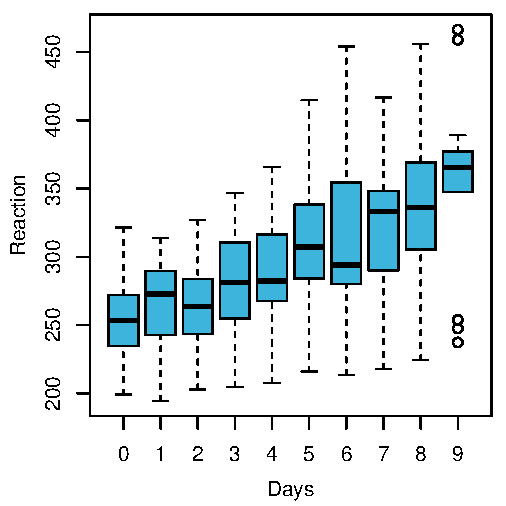
\includegraphics[scale=.8]{../figures/sleep_box}
    \end{column}
    \begin{column}{.55\textwidth}
\begin{lstlisting}
boxplot(Reaction ~ Days, sleepstudy)
\end{lstlisting}
    \end{column}
  \end{columns}
\end{frame}

\begin{frame}[fragile]{Visualization of individual data}
  \begin{columns}
    \begin{column}{.53\textwidth}
      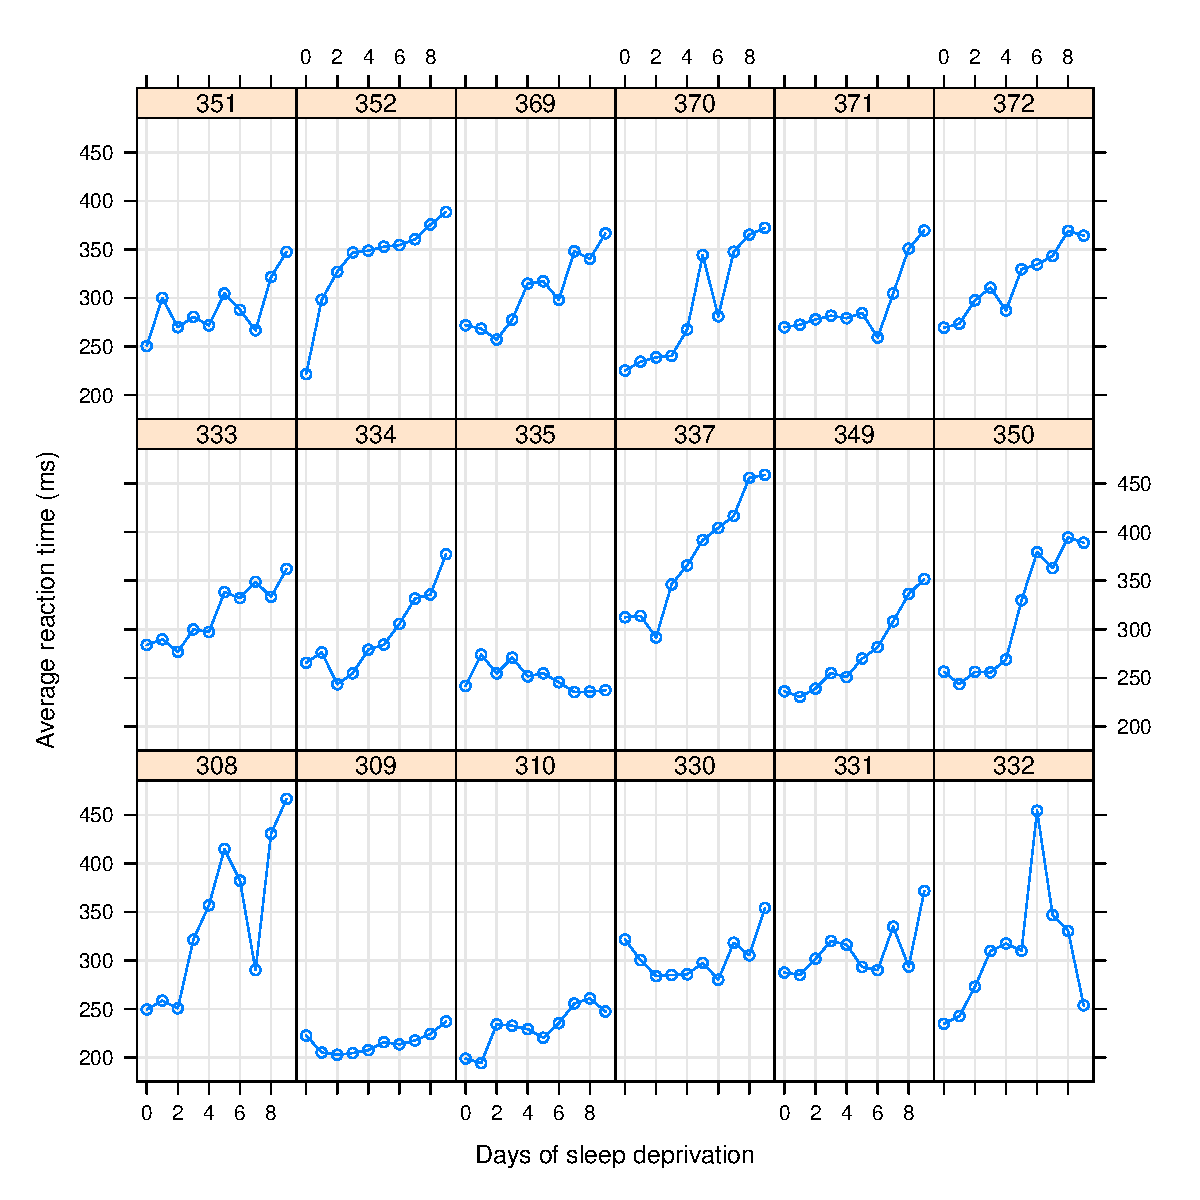
\includegraphics[scale=.5]{../figures/sleep_subjects}
    \end{column}
    \begin{column}{.55\textwidth}
\begin{lstlisting}
library(lattice)

xyplot(Reaction ~ Days | Subject,
  data = sleepstudy,
  type = c("g","b"),
  xlab = "Days of sleep deprivation",
  ylab = "Average reaction time (ms)",
  aspect = "xy")
\end{lstlisting}
    \end{column}
  \end{columns}
\end{frame}

\begin{frame}{Random intercept model}
  \begin{columns}
    \begin{column}{.5\textwidth}
  \begin{itemize}
\item The random intercept model adds a random intercept for each subject
\[
  y_{ij} = \beta_0 + \beta_1\,Days_{ij} + \upsilon_{0i} + \varepsilon_i
\]
with $\upsilon_{0i} \overset{iid}{\sim} N(0, \sigma^2_{\upsilon})$,
      $\varepsilon_{ij} \overset{iid}{\sim} N(0, \sigma^2)$
    \item The slope is identical for each subject (and the population)
  \end{itemize}
      \vspace{2.2cm}
    \end{column}
    \begin{column}{.5\textwidth}
      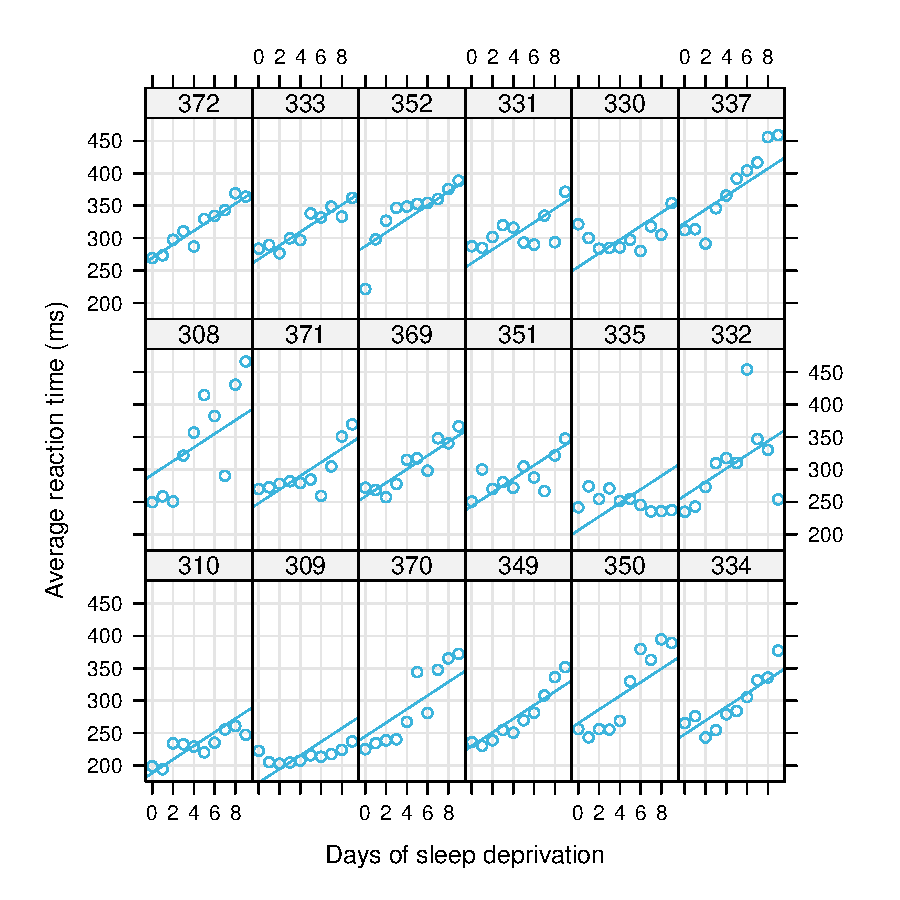
\includegraphics[scale=.5]{../figures/sleep_random_intercept}
    \end{column}
  \end{columns}
\end{frame}

% \begin{align*}
% \text{(Level 1)}  \quad y_{ij} &= b_{0i} + b_{1i}\,Days_{ij} + \varepsilon_{ij}\\
% \text{(Level 2)}  \quad b_{0i} &= \beta_0 + \upsilon_{0i}\\
%                   \quad b_{1i} &= \beta_1\\
% \text{(2) in (1)} \quad y_{ij} &= \beta_0 + \beta_1\,Days_{ij} +
%                                   \upsilon_{0i} + \varepsilon_{ij}
% \end{align*}
% \vfill
% with $\upsilon_{0i} \sim N(0, \sigma^2_{\upsilon})$ i.i.d.,
% $\varepsilon_{ij} \sim N(0, \sigma^2)$ i.i.d., $\upsilon_{0i}$ and
% $\varepsilon_{ij}$ i.i.d.\\[2ex]
% \vfill

\begin{frame}[fragile]{Random intercept model}
\begin{lstlisting}
lme0 <- lmer(Reaction ~ Days + (1 | Subject), sleepstudy)
summary(lme0)

# model matrices
X <- model.matrix(~ Days, sleepstudy)
Z <- model.matrix(~ 0 + Subject, sleepstudy)

# coefficients
coef(lme0)
fixef(lme0)
ranef(lme0)
\end{lstlisting}
\end{frame}

\begin{frame}[fragile]{Random slope model}
  \begin{columns}
    \begin{column}{.5\textwidth}
  \begin{itemize}
\item The random slope model adds a random intercept and a random slope for each
  subject
\[
  y_{ij} = \beta_0 + \beta_1\,Days_{ij} + \upsilon_{0i} +
      \upsilon_{1i}\,Days_{ij} + \varepsilon_{ij}
\]
with
\begin{align*}
  \begin{pmatrix} \upsilon_{0i}\\ \upsilon_{1i} \end{pmatrix} &\overset{iid}{\sim}
    N \left(\begin{pmatrix} 0\\ 0 \end{pmatrix}, \, \gmat{\Sigma}_\upsilon =
      \begin{pmatrix}
        \sigma^2_{\upsilon_0} & \sigma_{\upsilon_0 \upsilon_1} \\
        \sigma_{\upsilon_0 \upsilon_1} & \sigma^2_{\upsilon_1} \\
      \end{pmatrix} \right)
    \\
  \varepsilon_{ij} & \overset{iid}{\sim} N(0, \sigma_{\varepsilon}^2)
\end{align*}
      \vspace{-.5cm}
    \item Individual slopes for each subject
  \end{itemize}
    \end{column}
    \begin{column}{.5\textwidth}
      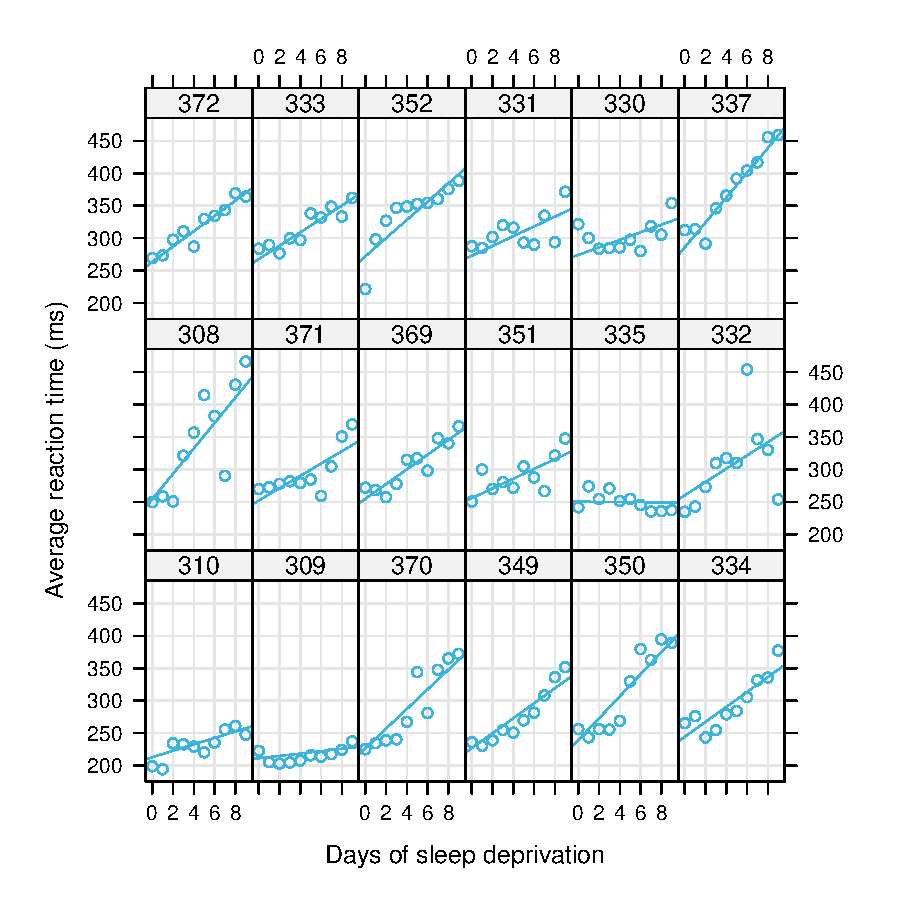
\includegraphics[scale=.5]{../figures/sleep_random_slope}
    \end{column}
  \end{columns}
\end{frame}

\begin{frame}[fragile]{Random slope model}
\begin{lstlisting}
lme1 <- lmer(Reaction ~ Days + (Days | Subject), sleepstudy)
summary(lme1)

# model matrices
X <- model.matrix(~ Days, sleepstudy)
Z <- model.matrix(~ 0 + Subject + Subject:Days, sleepstudy)

# coefficients
coef(lme1)
fixef(lme1)
ranef(lme1)
\end{lstlisting}
\end{frame}

\begin{frame}[fragile]{Model with uncorrelated random effects}
  \begin{itemize}
    \item We will now consider a model without correlated random effects
  \[
    y_{ij} = \beta_0 + \beta_1 Days_{ij} + \upsilon_{0i} + \upsilon_{1i} Days_{ij} +
    \varepsilon_{ij}
  \]
with
      \[
  \gvect{\upsilon}  \overset{iid}{\sim} N\left(\gvect{0}, \gmat{\Sigma}_{\upsilon} = 
    \begin{pmatrix}
      \sigma^2_{\upsilon_0} & 0 \\
      0 & \sigma^2_{\upsilon_1} \\
    \end{pmatrix}\right) ~~~\text{and}~~~
  \varepsilon_{ij}  \overset{iid}{\sim} N(0, \sigma_{\varepsilon}^2)
\]
  \end{itemize}
  \begin{lstlisting}
lme2 <- lmer(Reaction ~ Days + (Days || Subject), sleepstudy)
summary(lme2)

# likelihood-ratio test
anova(lme1, lme2)
# confidence intervals
confint(lme2)
  \end{lstlisting}
\end{frame}

\begin{frame}{Confidence intervals and interpretation}
  \begin{itemize}
    \item The results indicate that the extra parameter
      $\sigma_{\upsilon_0\upsilon_1}$ does not produce a significantly
      better fit
    \item Results show that we have a significant effect for days with an
  average increase in reaction time of 10.47\,ms for each day of sleep
  deprivation
    \item We get an estimate of $\sigma_{\upsilon_0} = 24.17$ for the
      standard deviation of reaction time for subjects and a standard
      deviation of $\sigma_{\upsilon_1} = 5.80$ for the dependence of
      reaction time on days of sleep deprivation
  \end{itemize}
\end{frame}

\begin{frame}[fragile]{Examining random effects and predictions}
      \begin{lstlisting}
coef(lme2)
fixef(lme2)
ranef(lme2)

# correlational structure for intercepts and slopes
dotplot(ranef(lme2, condVar = TRUE),
        scales = list(x = list(relation = "free")))[[1]]

# predictions for all subjects
predict(lme2)
      \end{lstlisting}
\end{frame}

\begin{frame}[fragile]{Examining random effects and predictions}
  \begin{center}
    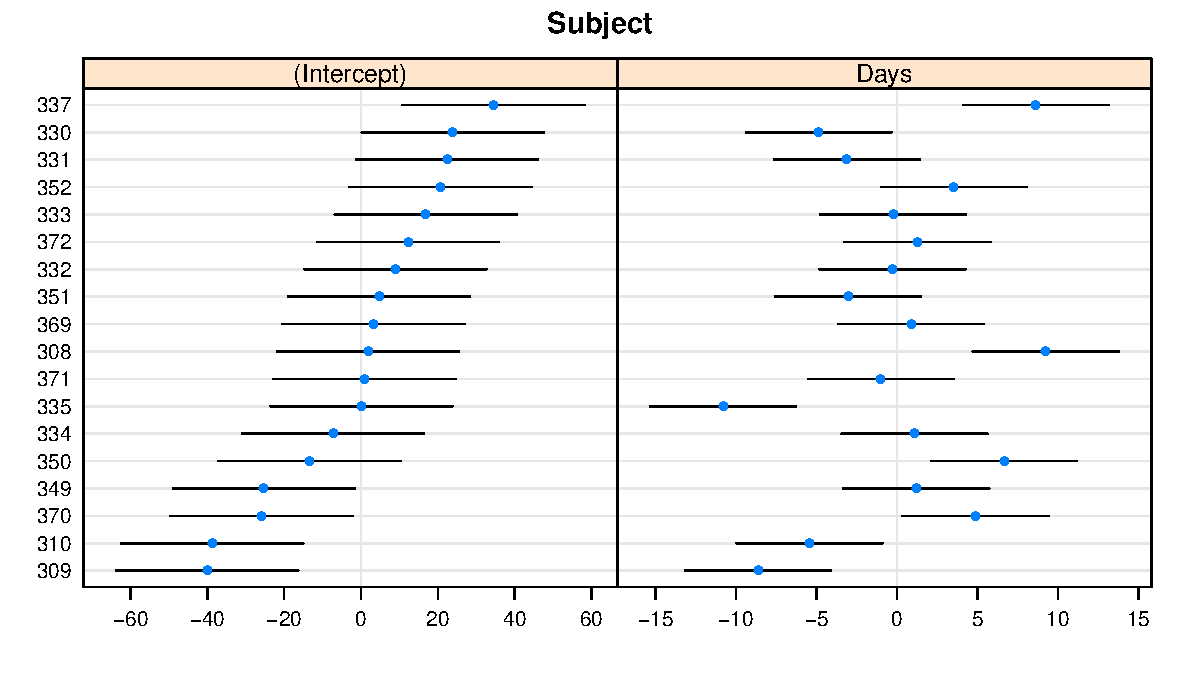
\includegraphics[scale=.6]{../figures/sleep_caterpillar}
  \end{center}
\end{frame}

\begin{frame}{Examining random effects and predictions}
  \begin{columns}
    \begin{column}{.5\textwidth}
      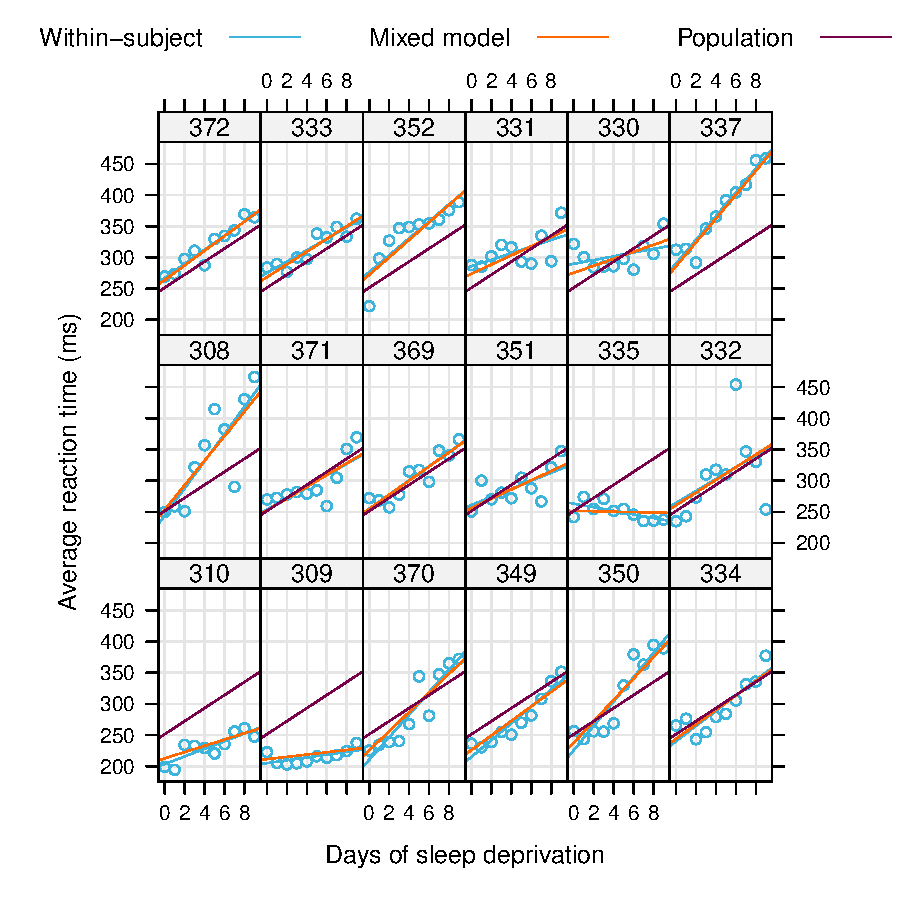
\includegraphics[scale=.5]{../figures/sleep_shrinkfit}
    \end{column}
    \begin{column}{.5\textwidth}
      \begin{itemize}
        \item Within-subject regression line shows regression line fitted to
          data for each individual
        \item Population regression line shows fixed effects for mixed-effects
          model
        \item Mixed model regression line shows individual regression lines as
          predicted by mixed-effects models
      \end{itemize}
    \end{column}
  \end{columns}
\end{frame}

\begin{frame}{Shrinkage}
  \begin{columns}
    \begin{column}{.5\textwidth}
  \begin{itemize}
    \item When per-subject slopes and intercepts calculated from a
      mixed-effects model are compared to estimated slopes and intercepts
      within subjects, estimates from mixed-effects model are
      closer to the population estimates (the fixed effects)
    \item This pattern is sometimes described as {\it shrinkage} of
      coefficients toward the population values
    \item The more within-subject variance, the stronger parameters {\it shrink}
      towards the population parameters
    % \item In a mixed-effects model, we assume that the levels of a grouping
    %   factor are a selection from a population and, as a result, can be
    %   expected to share characteristics to some degree
  \end{itemize}
    \end{column}
    \begin{column}{.5\textwidth}
    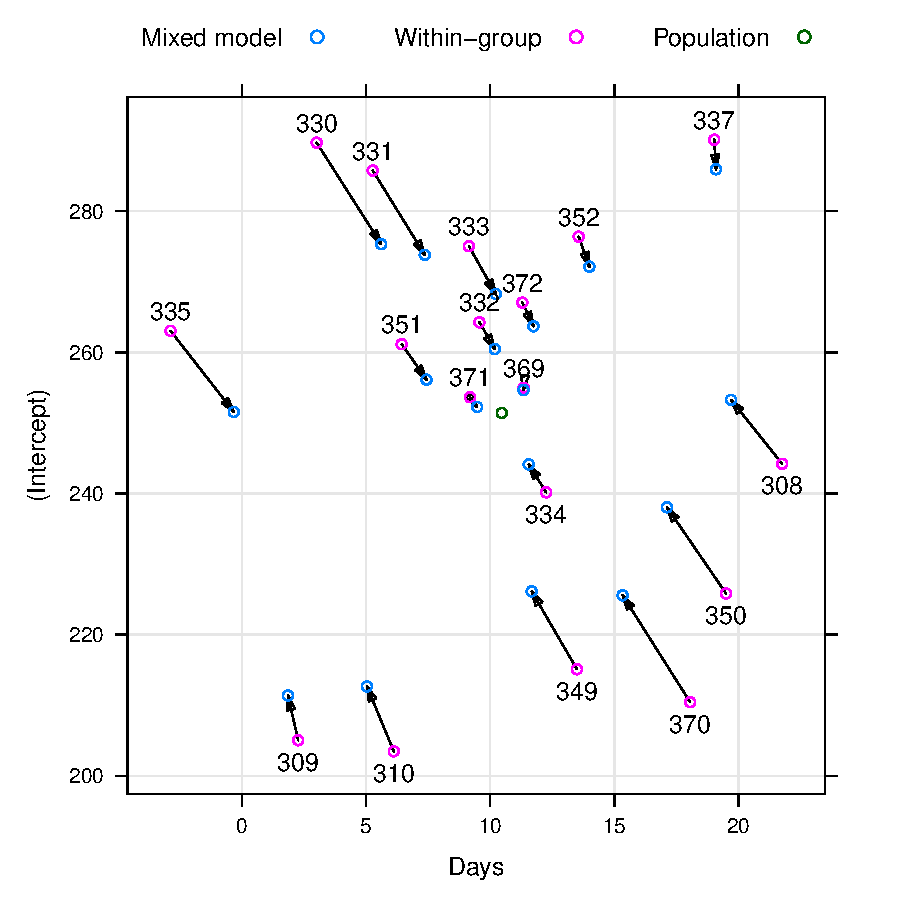
\includegraphics[scale=.48]{../figures/sleep_shrinkage}
    \end{column}
  \end{columns}
\end{frame}

\begin{frame}[fragile]{Assumptions}
  \begin{columns}
    \begin{column}{.5\textwidth}
      \begin{itemize}
        \item Assumptions can be checked visually
        \item Normality assumption
          \begin{lstlisting}
qqmath(lme2,
     col = sleepstudy$Subject,
     pch = sleepstudy$Days)
          \end{lstlisting}
        \item Independence assumption
          \begin{lstlisting}
plot(lme2,
     col = sleepstudy$Subject,
     pch = sleepstudy$Days)
          \end{lstlisting}
      \end{itemize}
      {\tiny \url{https://bbolker.github.io/morelia_2018/notes/mixedlab.html}}
    \end{column}
    \begin{column}{.5\textwidth}
      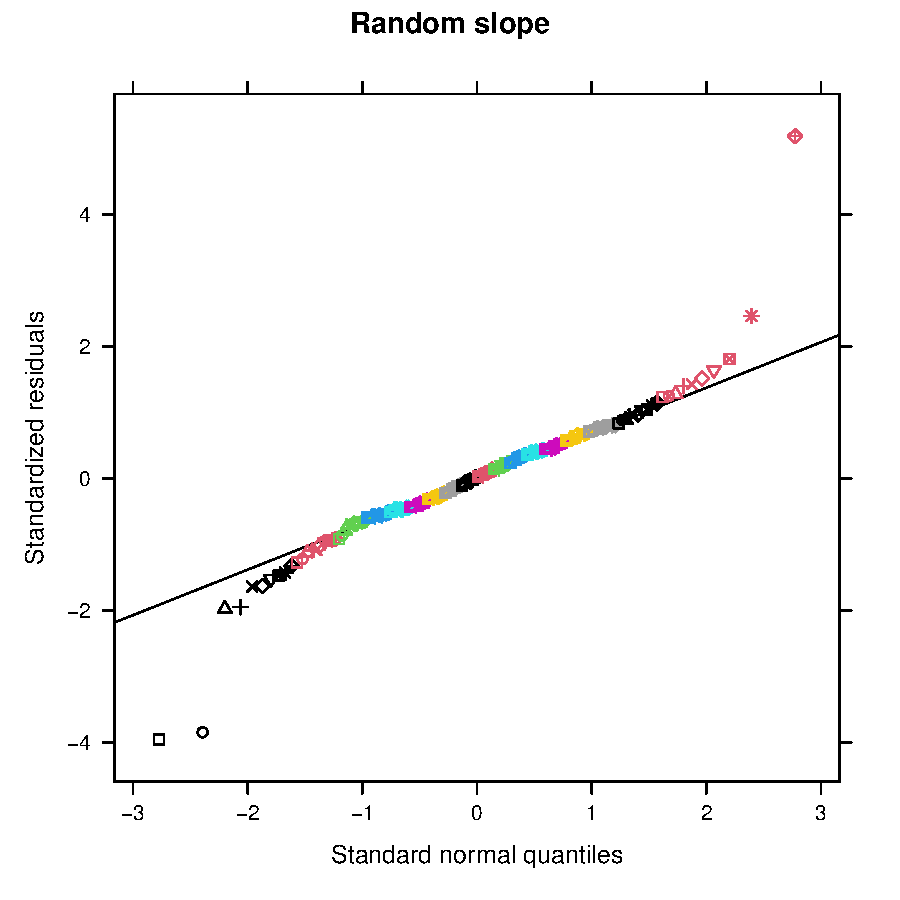
\includegraphics[scale=.5]{../figures/assump_qqplot_slope.pdf}
    \end{column}
  \end{columns}
\end{frame}

\begin{frame}{Assumptions}
  \begin{columns}
    \begin{column}{.5\textwidth}
      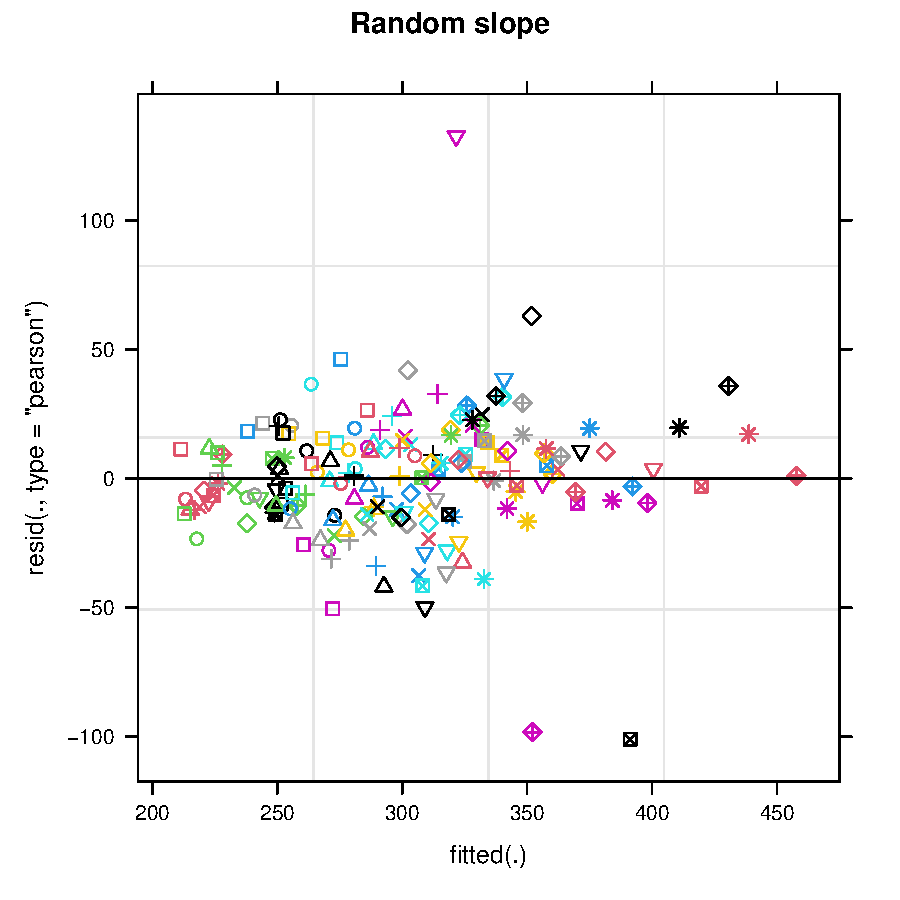
\includegraphics[scale=.5]{../figures/assump_resid_slope.pdf}
    \end{column}
    \begin{column}{.5\textwidth}
      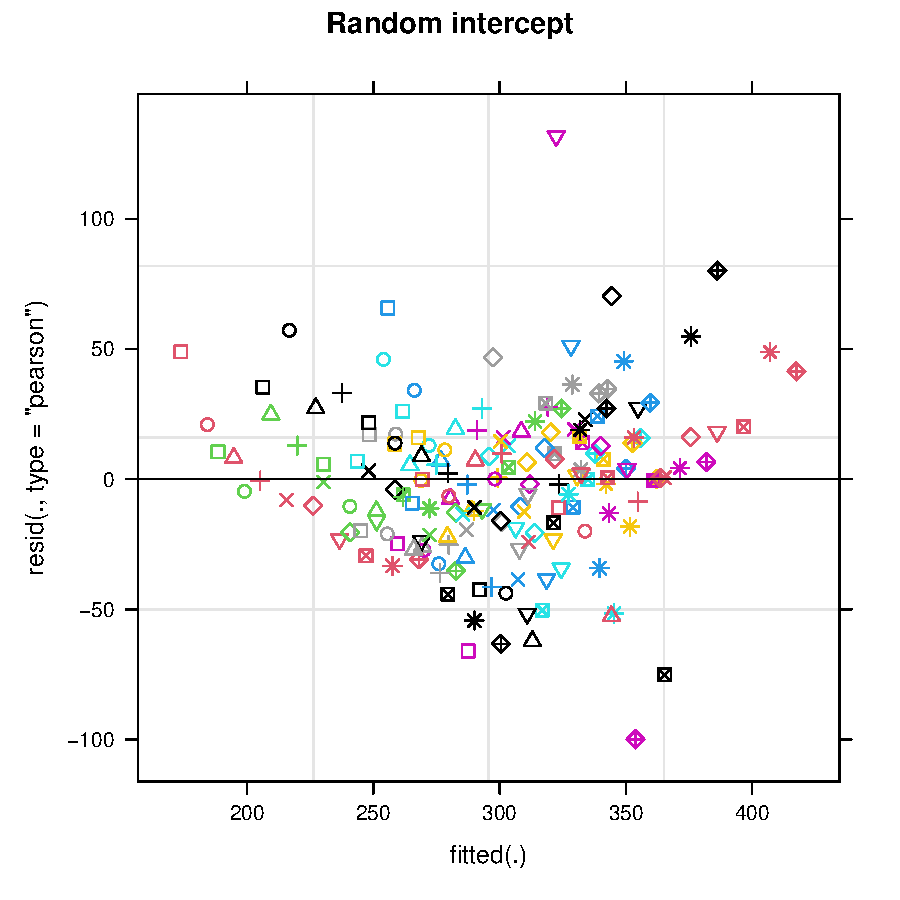
\includegraphics[scale=.5]{../figures/assump_resid_intercept.pdf}
    \end{column}
  \end{columns}
\end{frame}

\section{Parameter estimation}

\begin{frame}{Maximum Likelihood Estimation}
  \begin{itemize}
    \item The maximum likelihood principle was introduced by
      R.\,A.\ Fisher
      \begin{itemize}
      \item It can be used for almost all estimation problems, also complex
        ones
      \item The resulting estimation functions have many desirable
        properties
      \end{itemize}
    \item Obtaining the MLE $\hat{\vartheta}$ takes the
      following steps\\[1ex]
    \begin{enumerate}
      \item Generate the log-likelihood
      \[
        \log L(\vartheta)
      \]
      \vspace{-3ex}
      \item Take the derivative of the log-likelihood with respect to
        parameter $\vartheta$
      \[
        (\log L)' (\vartheta) = \frac{d \log L(\vartheta)}{d \vartheta}
      \]
      \vspace{-3ex}
      \item Set the derivative equal to 0
      \[
        (\log L)' (\hat{\vartheta}) = 0
      \]
      \vspace{-3ex}
      \item Solve the resulting equation for the estimator $\hat{\vartheta}$
    \end{enumerate}
  \end{itemize}
\end{frame}

\begin{frame}{Restricted Maximum Likelihood Estimation}
  \begin{itemize}
    \item The restricted maximum likelihood (REML) approach is a form of Maximum
      Likelihood Estimation
    \item In particular, REML is used as a method for fitting linear
      mixed-effects models
    \item In contrast to traditional Maximum Likelihood Estimation, REML can
      produce unbiased estimates of variance and covariance parameters
    \item MLE and REML do not outmatch each other, both can be used
    \item REML is the default in \texttt{lme4}, but if we want to conduct
      likelihood ratio tests, only MLE estimates are valid
  \end{itemize}
\end{frame}

% \begin{frame}[fragile]{}
%   \begin{block}{Exercise}
%     \begin{itemize}
%       \item 
%     \end{itemize}
%   \end{block}
% \end{frame}

\appendix

%\begin{frame}[allowframebreaks]{References}
\begin{frame}{References}
%\renewcommand{\bibfont}{\footnotesize}
  \printbibliography
  \vfill
\end{frame}

\end{document}

